\chapter{The Polar Front as a major biogeographic boundary in the Southern Ocean} 
\label{ch:polarfront}

Sections of this chapter have been previously published in \bibentry{Wilkins:2012td}.

\section{Summary}

\section{Introduction}


\section{Methods}
\subsection{Sampling and metagenomic sequencing}

Sampling\footnote{Sampling was performed by Jeffrey M. Hoffman and Jeffrey B. Mcquaid} was conducted on board the RSV \emph{Aurora Australis} during cruise V3 \ac{CEAMARC/CASO} from 13 December 2007 -- 26 January 2008. 
This cruise occupied the SR3 latitudinal transect from Hobart, Australia (44\textdegree{} S) to the Mertz Glacier, Antarctica (67\textdegree{} S) within a longitudinal range of 140--150\textdegree{} E.
Nineteen samples (16 surface, 3 deep) were obtained along almost the entire latitudinal range \figref{fig:samplemap}.

% the sample map
\begin{figure}[!ht]
  \centering
  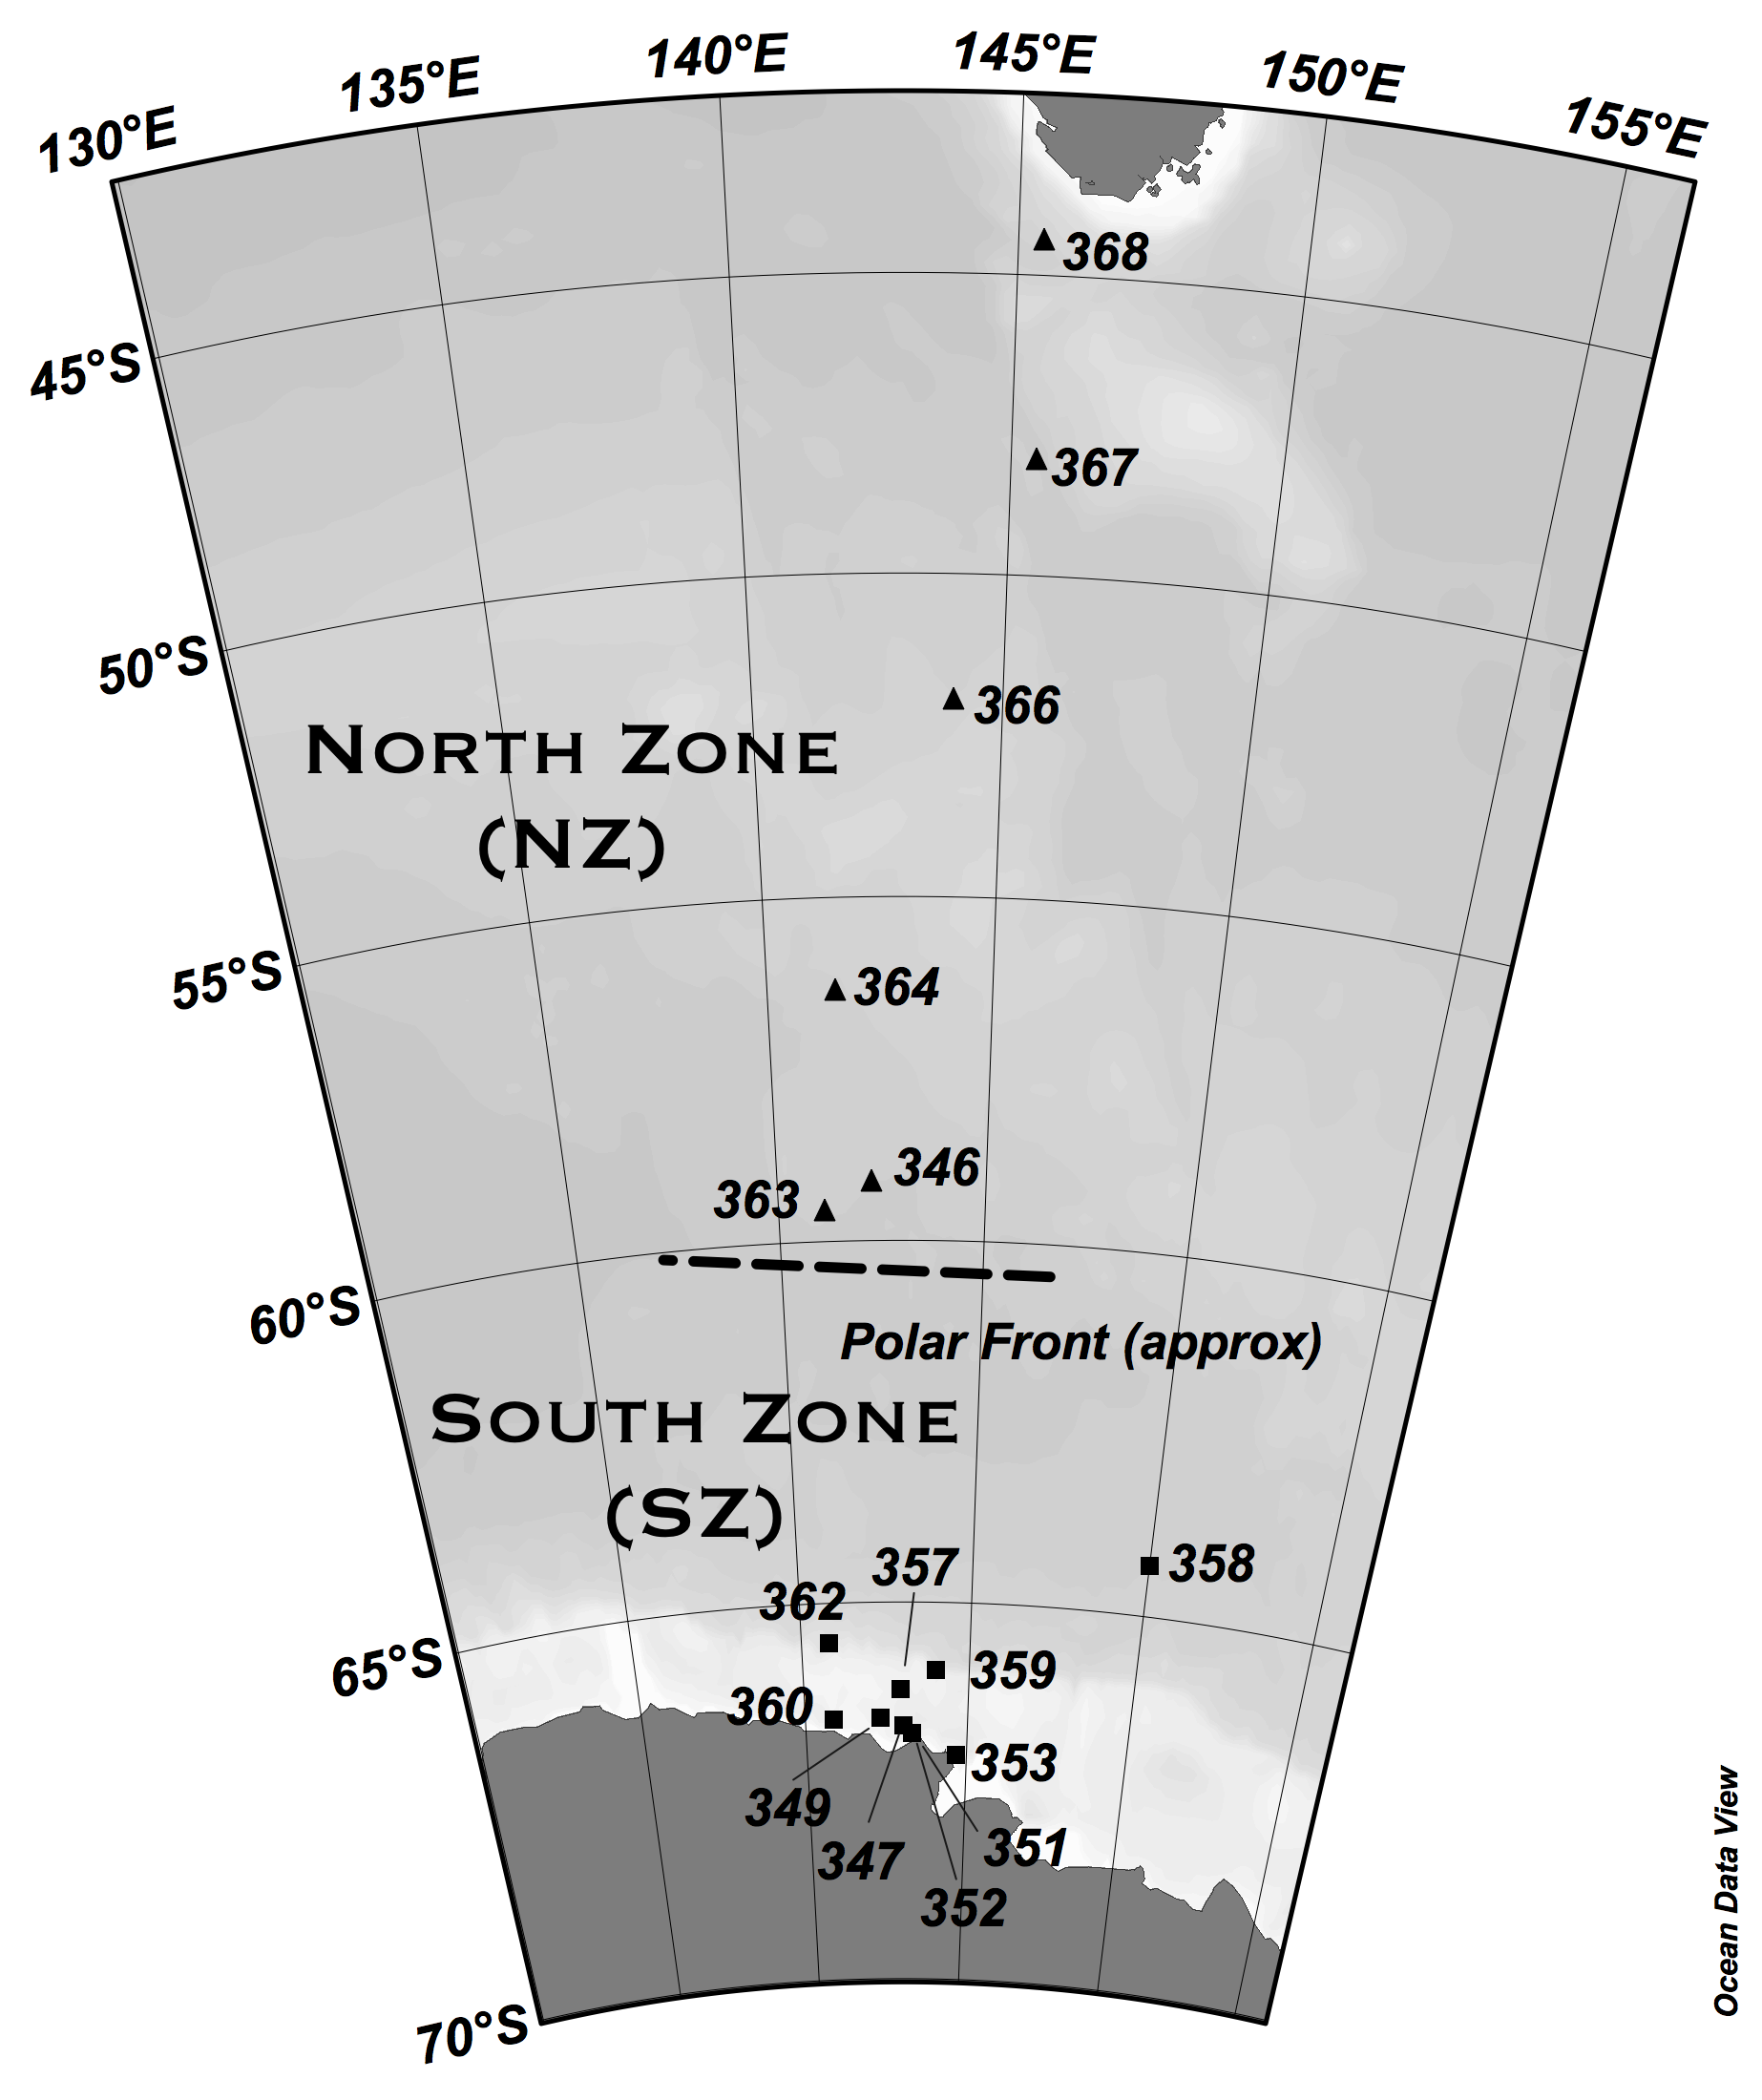
\includegraphics[width=\textwidth]{../polarfront/samplemap.png}
  \caption[Map showing sites of seawater samples used in the Polar Front study]{Sites of seawater samples used in this study. 
  Squares indicate surface samples from the North Zone; crosses samples from the South Zone. 
  The dashed line represents the Polar Front.}
  \label{fig:samplemap}
\end{figure}


A range of data were recorded by integrated instruments on the RSV \emph{Aurora Australis} including location, water column depth, water temperature, salinity, fluorescence and meterological data \tabref{tab:samplelist}.
These data were used to locate the \ac{PFZ} based on a surface temperature gradient of $\sim$ 1.35 \textdegree{}C across a distance of 45--65 km, placing the \ac{PF} at approximately $-59.70$\textdegree{} of latitude, consistant with previous descriptions \cite{Moore:1999to,Sokolov:2002tc}.
Samples were accordingly grouped into ``North'' and ``South'' zones, while the three deep samples composed a ``Deep'' zone \tabref{tab:samplelist}.
The \ac{NZ} represents waters from the Subtropical, Subantarctic and \ac{PFZ} regions, while the \ac{SZ} represents the \ac{AZ}.

\begin{sidewaystable}
\sffamily
\caption[Details of samples used in Polar Front study]{\sffamily{}Sampling time, location and physicochemical properties of samples used in this study.
All data were retrieved from underway instruments aboard the RSV \textit{Aurora Australis}.}
\label{tab:samplelist}
\smallskip
\begin{tabularx}{\textheight}{lllXXXXXXXX}
\toprule
\textbf{Sample} & \textbf{Zone} & \textbf{Date} & \textbf{Latitude} & \textbf{Longitude} & \textbf{Water \linebreak Column \linebreak Depth (m)} & \textbf{Sample Depth (m)} & \textbf{Temperature (\textdegree{}C)} & \textbf{Salinity (PSU)} & \textbf{Fluorescence \linebreak (\textmu{}gL\textsuperscript{\textminus{}1})} & \textbf{Volume \linebreak filtered (L)}\\
\midrule

346 & North & 20/12/2007 & \textminus{}59.31 & 142.59 & 4294 & 2 & 2.9 & 33.75 & 0.3 & 500\\
347 & South & 23/12/2007 & \textminus{}66.02 & 142.74 & 450 & 2 & 0.6 & 34.20 & 4.0 & 250\\
349 & South & 27/12/2007 & \textminus{}66.57 & 142.32 & 370 & 1.5 & \textminus{}1.3 & 34.40 & 2.3 & 250\\
351 & South & 28/12/2007 & \textminus{}66.56 & 143.43 & 823 & 1.5 & \textminus{}0.6 & 34.30 & 1.3 & 500\\
352 & South & 29/12/2007 & \textminus{}66.77 & 143.32 & 164 & 2.5 & \textminus{}0.8 & 34.30 & 3.1 & 500\\
353 & South & 30/12/2007 & \textminus{}67.05 & 144.68 & 180 & 2 & \textminus{}1.8 & 34.40 & 0.3 & 500\\
357 & South & 05/01/2008 & \textminus{}66.17 & 143.02 & 580 & 2 & \textminus{}0.4 & 34.15 & 2.5 & 500\\
358 & South & 09/01/2008 & \textminus{}64.30 & 150.03 & 3550 & 2 & 0 & 33.55 & 0.5 & 500\\
359 & South & 12/01/2008 & \textminus{}66.19 & 143.53 & 540 & 2 & \textminus{}0.2 & 34.21 & 2.5 & 500\\
360 & South & 13/01/2008 & \textminus{}66.58 & 141.02 & 316 & 2 & \textminus{}0.7 & 34.04 & 6.2 & 500\\
362 & South & 19/01/2008 & \textminus{}65.54 & 140.83 & 1064 & 2 & 0.7 & 32.20 & 0.5 & 500\\
363 & North & 22/01/2008 & \textminus{}60.00 & 141.31 & 4473 & 2 & 3.3 & 33.77 & 0.1 & 500\\
364 & North & 23/01/2008 & \textminus{}56.70 & 141.88 & 3693 & 2 & 4 & 33.70 & 0.5 & 500\\
366 & North & 24/01/2008 & \textminus{}52.02 & 144.14 & 3180 & 2 & 7.6 & 33.84 & 0.3 & 500\\
367 & North & 25/01/2008 & \textminus{}48.25 & 145.90 & 3490 & 2 & 11 & 34.43 & 0.2 & 500\\
368 & North & 26/01/2008 & \textminus{}44.72 & 145.78 & 3201 & 2 & 14.8 & 34.96 & 1.3 & 560\\

\bottomrule
\end{tabularx}
\end{sidewaystable}


At each station, $\sim$ 250--560 L of seawater was pumped from $\sim$ 1.5--2.5 m below the sea surface into drums stored at ambient temperature on deck. 
In the case of deep samples, $\sim$ 225--230 L of seawater was collected from Niskin bottles attached to a \ac{CTD} (SeaBird, Bellevue, USA).
Seawater samples were prefiltered through a 20 \textmu{}m plankton net, then filtrate was captured on sequential 3.0 \textmu{}m, 0.8 \textmu{}m and 0.1 \textmu{}m polyethersulfone membrane filters (Port Washington, USA), and immediately stored at $-20$ $^\circ$C \cite{Rusch:2007ez,Ng:2010cd}.

DNA extraction\footnote{DNA extraction was performed by Cynthia Andrews-Pfannkoch and others at the J. Craig Venter Institute} was performed at the J. Craig Venter Institute (Rockville, USA) as described in \citet{Rusch:2007ez}.
Pyrosequencing was performed on a GS20 FLX Titanium instrument (Roche, Branford, USA) also at the J. Craig Venter Institute as described in \citet{Lauro:2010jna}.
Duplicate reads and reads with many pyrosequencing errors were removed as described in \citet{Lauro:2010jna}.

\subsection{Phylogenetic analysis of metagenomic data}

\subsubsection{\softwarename{blast} analysis}

A subset of the RefSeq microbial (bacterial and archaeal) genome database (release 41, retrieved May 31 2012 from \url{ftp://ftp.ncbi.nih.gov/refseq/release/}) was prepared by excluding sequences with the words ``shotgun'', ``contig'', ``partial'', ``end'' or ``part'' in their headers \cite{Angly:2009ip}.
Because this database was not expected to contain representative genomes for every species present, \acp{OTU} in this study are defined by the best species match to this database, and may for example represent congeners.

The metagenomic reads from each sample were compared against this database using \softwarename{tblastx}, with default parameters except for: E-value threshold $1.0\times{}10^{-3}$, cost to open gap 11, cost to extend gap 1, masking of query sequence by \softwarename{SEG} masking with lookup table only.

\subsubsection{Identification of minimal species sets with \softwarename{minspec}}

A computational method to minimise false \ac{OTU} identifications and increase the accuracy of \ac{OTU} abundance estimates (\softwarename{minspec}) was developed and implemented in \softwarename{perl}.
Following the approach of \citet{Ye:2009bl} to the parsimonious reconstruction of biochemical pathways (\softwarename{MinPath}), \softwarename{minspec} computes the smallest set of OTUs sufficient to explain a set of observed high-quality hits against RefSeq (or any other sequence database).
The minimal set computation is framed as a linear programming problem and solved with the \ac{GLPK} tool \ac{GLPSOL} (Free Software Foundation, Boston).
This approach eliminates many of the spurious \ac{OTU} identifications which result from reads with strong identity to more than one \ac{OTU}. 
The ``minimal species set'' is liable to exclude some low-abundance \acp{OTU}, but gives more faithful abundance estimates and eliminates many false positives.

To validate this approach and estimate error rates, an assemblage of hypothetical taxa was simulated with varying degrees of overlapping genomic identity and a logarithmic rank-abundance curve. 
A simulated metagenomic sampling and \softwarename{blast} search was performed on this set, and the results processed with \softwarename{minspec}.
The outputs of all \softwarename{tblastx} searches against RefSeq were processed by \softwarename{minspec}, and hits not belonging to the minimal sets were removed.

TODO HERE 



\subsection{Functional analysis of metagenomic data}

\section{Results}
\subsection{Metagenomic sequencing}
\subsection{Phylogenetic analysis of metagenomic data}
\subsubsection{Validation of \softwarename{minspec}}
\subsection{Functional analysis of metagenomic data}

\section{Discussion}

\section{Conclusions}

